\newpage
\setheaders{Tutorials}{\daydateyear}
\section{Tutorials}
\index{Kar, Sudipta}
\index{S\'anchez, Danae}
\index{Fikri Aji, Alham}
\index{Mijangos, V\'ictor}

% Tutorial A
\begin{center}
{\bfseries\Large Training Lightweight Model via Knowledge Distillation and Parameter Efficient Finetuning} \\
\vspace{1.0em}
{\large\bf Alham Fikri Aji} \\

\textbf{\daydateyear{}, 09:00--10:30 and 10:30--12:00 CST}\\
\textbf{Do\~na Adelita}\\
\textbf{English}
\end{center}

\begin{center}
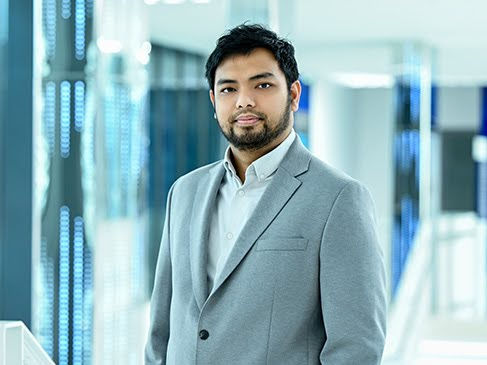
\includegraphics[width=0.4\linewidth]{content/mexican_nlp/alham.jpeg}
\end{center}

{\bfseries Abstract:}
Language models can be resource-hungry and prohibitive to train and deploy for many people due to a lack of proper computing resources. In this tutorial, we delve into how to build smaller, more lightweight models without sacrificing quality via knowledge distillation. Additionally, we delve into training your model with less memory usage through parameter-efficient finetuning. In this tutorial, we will delve into the hands-on implementation. It is ideal for those just delving into the field of AI/NLP.

{\bfseries Biography:}
Alham Fikri Aji is an Assistant Professor at MBZUAI, holding a Ph.D. from the University of Edinburgh's Institute for Language, Cognition, and Computation. His doctoral research, supervised by Dr. Kenneth Heafield and Dr. Rico Sennrich, focused on enhancing the training and inference speed of machine translation. Dr. Aji's current research centers around multilingual, low-resource, and low-compute Natural Language Processing (NLP). His recent work has been in developing diverse multilingual large language models. and multilingual NLP resources, particularly for underrepresented languages, with a specific emphasis on Indonesian. He has worked at Amazon, Google, and Apple in the past.
% End tutorial A

\clearpage
% Tutorial B
\begin{center}
{\bfseries\Large Introduction to Attention Mechanisms in Transformers} \\
\vspace{1.0em}
{\large\bf V\'ictor Mijangos} \\

\textbf{\daydateyear{}, 09:00--10:30 and 10:30--12:00 CST}\\
\textbf{Don Juli\'an}\\
\textbf{Espa\~nol}
\end{center}

\begin{center}

\includegraphics[width=0.4\linewidth]{content/mexican_nlp/victor.jpeg}
\end{center}

{\bfseries Abstract:}
Attention layers are currently central mechanisms in language models. Transformers, which represent the state of the art in this field, rely on the use of attention layers in combination with other strategies. Attention has also been used in models based on sequence-to-sequence recurrent networks, providing significant improvements in natural language processing tasks such as machine translation and text generation. Understanding how these mechanisms work is essential to comprehend current language models. This workshop aims to present a first approach to the attention mechanisms used in neural networks. Firstly, the basic theoretical concepts to understand attention and its operation will be presented, other attention mechanisms, mainly sparse attention, will be reviewed, and the relationship of attention with auto-encoded and auto-regressive language models will be discussed. Finally, its relationship with other mechanisms such as convolutional layers and graph layers, highlighting their advantages and disadvantages, will be addressed. Secondly, the technical principles for the implementation of attention mechanisms in Pytorch and their incorporation within the architecture of Transformers will be covered.

{\bfseries Biography:}
V\'ictor Mijangos de la Cruz is a Full-Time Professor at the Faculty of Sciences, where he teaches subjects related to Artificial Intelligence, Neural Networks, and Computational Linguistics. In addition to teaching, he develops research projects aimed at exploring inductive biases in neural networks and the application of deep learning models for the development of technologies in indigenous languages. His interests lie in the study of the capabilities and limitations of deep learning, computational linguistics, and the creation of technologies for indigenous languages, particularly in the Otomí language.
% End tutorial B


\clearpage
% Tutorial C
\begin{center}
{\bfseries\Large Exploring Transformers and Limitations in Language Modeling} \\
\vspace{1.0em}
{\large\bf Danae Sánchez} \\

\textbf{\daydateyear{}, 14:00--16:00 CST}\\
\textbf{Do\~na Adelita}\\
\textbf{Espa\~nol}
\end{center}

\begin{center}
    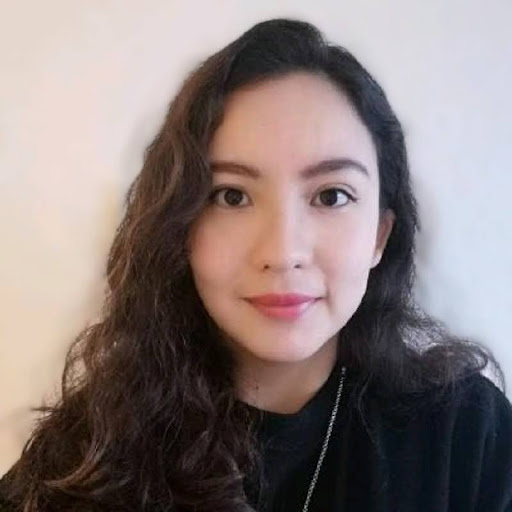
\includegraphics[width=0.4\linewidth]{content/mexican_nlp/danae.jpeg}
\end{center}

{\bfseries Abstract:}
This tutorial explores language modeling techniques in Natural Language Processing (NLP), covering key concepts from traditional approaches to Transformer architectures. Beginning with an introduction to NLP and language modeling, it delves into probabilistic language models and progresses to neural language models, emphasizing the significance of embeddings for semantic representation. Moving on to Transformer models, we will discuss key concepts such as multi-head attention mechanisms, masked language modeling, and encoder models. Additionally, the tutorial addresses the limitations of large language models, providing insights into challenges and considerations for leveraging these models effectively in practical applications.

{\bfseries Biography:}
Danae Sánchez Villegas is a postdoctoral researcher at the University of Copenhagen. She holds a Ph.D. and a Master's degree in Computer Science from the University of Sheffield and a Bachelor's degree in Computer Engineering from the Instituto Tecnológico Autónomo de México. Her research interests include multilingual natural language understanding, vision and language modeling, and computational social science. Danae has worked as a Research Associate in the Natural Language Processing Group at the University of Sheffield and as an Applied Scientist Intern at Amazon Alexa.
% End tutorial C
\clearpage

% Tutorial D
\begin{center}
{\bfseries\Large The Power of Rewards - Reinforcing Language Models with Reinforcement Learning} \\
\vspace{1.0em}
{\large\bf Sudipta Kar} \\

\textbf{\daydateyear{}, 14:00--16:00 CST}\\
\textbf{Don Juli\'an}\\
\textbf{English}
\end{center}

\begin{center}
    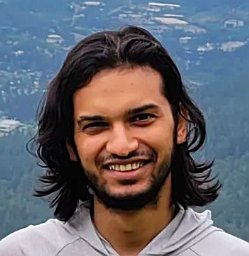
\includegraphics[width=0.4\linewidth]{content/mexican_nlp/sudipta.jpeg}
\end{center}

{\bfseries Abstract:}
Language models ranging from BERT to GPT have shown impressive performance on many natural language tasks through first self-supervised pre-training on large text corpora and then fine-tuning on downstream tasks or even with zero-shot or few-shot approaches. These models are also very powerful in solving multiple tasks. However, their capabilities are still limited as they lack a built-in reward signal to directly optimize for the end task objective or align to certain human preferences.On the other hand, Reinforcement Learning (RL) is another area in machine learning which is commonly applied to develop systems that improve over real-time feedback loops (such as games). Because it provides a framework for optimizing goal-directed behavior through rewards. In this tutorial, we will explore how reinforcement learning came into the play of language modeling and suddenly changed the game by reinforcing the representational power of large language models with the ability to more efficiently solve tasks requiring reasoning, planning, and knowledge. We will first provide background on contemporary language models and reinforcement learning fundamentals. Next, we will discuss techniques for applying policy gradient methods to fine-tune language models to maximize rewards from an environment. Attendees will learn how to practically apply RL to language tasks, understand tradeoffs between different algorithms, and gain insight into state-of-the-art research in this emerging field.

{\bfseries Biography:}
Sudipta Kar is a Senior Applied Scientist at Amazon AGI. He received his Ph.D. in Computer Science from the University of Houston in 2020 under the supervision of Thamar Solorio. His doctoral research focused on creative text analysis. Currently, he works on developing intelligent systems to enable seamless proactivity in smart voice assistants such as Alexa. His research interests include computational systems for low-resource languages, language models, and information extraction. He has co-organized multiple natural language processing workshops and shared tasks, including BLP, CALCS, MultiCoNER, and SentiMix. Additionally, in 2023 he led the first NLP hackathon held in Bangladesh.
% End tutorial D



\newpage
